% ============================================================
%  MILESTONE 5 (M5) -- FULL COMBINED SEMINAR PAPER
%  Topic : High-Level Synthesis with Game Theoretic Scheduling
%  Author: Sumon Boiddo (ID 2220054) | HSHL
%  Course: HW/SW Co-Design Seminar
%
%  This is the final combined seminar paper, integrating the
%  content developed across milestones M1-M4 into one coherent
%  IEEE-format document. All ideas originate from the author's
%  own seminar work; benchmark data is cited from Murugavel and
%  Ranganathan (IEEE TVLSI 2003). AI usage is disclosed in the
%  accompanying JSON and BibTeX protocols.
% ============================================================

\documentclass[conference]{IEEEtran}
\IEEEoverridecommandlockouts
\usepackage{amsmath,amssymb,amsfonts}
\usepackage{graphicx}
\usepackage{xcolor}
\usepackage{booktabs}
\usepackage{tikz}
\usetikzlibrary{positioning,arrows.meta,shapes.geometric}

\begin{document}

\title{High-Level Synthesis with Game Theoretic Scheduling}

\author{\IEEEauthorblockN{Sumon Boiddo}
\IEEEauthorblockA{\textit{Student ID: 2220054}\\
\textit{Hochschule Hamm-Lippstadt}\\
Lippstadt, Germany\\
sumon.boiddo@stud.hshl.de}}

\maketitle

\begin{abstract}
Power consumption has become a critical design dimension in modern
VLSI circuits, particularly for battery-powered and embedded systems.
This seminar paper presents a game theoretic approach to the scheduling
and binding problems of High-Level Synthesis (HLS). In this approach,
a Data Flow Graph (DFG) determines which operations are assigned to
which control cycles, and each functional unit is modeled as a player
in a first-price sealed-bid auction. The Nash equilibrium is then
applied to select, for every operation, the functional unit with the
lowest power cost, thereby reducing switching activity and overall
power consumption. The techniques of functional unit sharing, path
balancing, and register assignment are incorporated to further reduce
unwanted computations. The approach reduces power without increasing
hardware area and with only a small latency cost. Benchmark data drawn
from Murugavel and Ranganathan~\cite{murugavel2003} indicate average
power improvements of about 6.3\% for scheduling, 13.9\% for binding,
and 11.8\% for combined scheduling and binding over linear and integer
linear programming baselines. The paper also discusses where this
method fits among prior low-power synthesis techniques, its tradeoffs,
its applications in IoT and mobile devices, and directions for future
work.
\end{abstract}

\begin{IEEEkeywords}
High-level synthesis, scheduling, binding, game theory, Nash
equilibrium, power optimization, behavioral synthesis.
\end{IEEEkeywords}

% ============================================================
\section{Introduction}

Power consumption in CMOS VLSI circuits has added an important
dimension to the design space, in addition to area and timing. The
spread of portable and wireless computing has increased the demand for
low-power yet high-performance circuits. Higher power consumption
shortens battery life in portable systems, increases packaging and
cooling costs, and reduces reliability; the reliability of a circuit
decreases by roughly 50\% for every $10\,^{\circ}\mathrm{C}$ rise in
temperature~\cite{small1994}. As a result, minimizing power has become
as important as meeting area and timing goals.

High-Level Synthesis (HLS) converts an algorithm-level description,
typically written in a language such as C or C++, directly into a
hardware design, rather than relying on manual gate-level
design~\cite{gajski1992}. This makes complex hardware feasible to
produce. The behavioral synthesis of computational units in HLS
proceeds through three main steps: \emph{scheduling}, which decides in
which control cycle each operation is executed; \emph{allocation},
which decides how many resources of each type are needed; and
\emph{binding}, which decides which specific hardware unit performs
each operation~\cite{benini2000}. Scheduling and binding strongly
influence the power, speed, latency, and hardware utilization of the
final circuit, and they waste the most power when handled poorly.

The main focus of this work is to solve the scheduling and binding
problem on a Data Flow Graph (DFG) using a game theoretic formulation,
such that power consumption is minimized without any increase in area
overhead. Although existing methods based on integer linear programming
(ILP) and linear programming (LP) can optimize power to some extent,
they are often complex and cannot always handle scheduling and binding
flexibly, especially when functional unit selection and switching
activity must be minimized at the same
time~\cite{shiue2000}. Game theory is well suited to this setting
because each hardware unit can be modeled as a player, and the Nash
equilibrium provides a stable assignment in which operations are
directed to the functional unit with the lowest power cost. The primary
goals are therefore to reduce power consumption, to avoid increasing
hardware area, and to make scheduling and binding decisions more
systematic.

This paper first represents operations and their data dependencies
using a DFG and then applies the Nash equilibrium to select a suitable
functional unit for each operation. It places this approach within the
landscape of prior low-power synthesis methods, analyzes its tradeoffs,
reports benchmark results, and discusses its advantages, limitations,
applications in IoT and mobile devices, and future improvements such as
latency optimization, interconnect binding, support for larger
circuits, and AI-based decision making.

% ============================================================
\section{Background and Problem Context}

\subsection{Sources of Power and the Role of Scheduling and Binding}
At the behavioral level, power is consumed mainly by computational
units (functional units and registers), by communication units, and by
peripheral units. Within HLS, poor scheduling leads to unnecessary
switching activity and therefore higher power and latency, while a poor
binding choice, such as selecting the wrong adder for an operation,
increases the switching activity of that unit and wastes power.
Allocation also matters: too many units increase area and power, while
too few increase latency. The problem addressed here is to assign
operations to hardware units so that the least power is wasted, without
increasing chip area or causing large latency increases.

\subsection{Prior Low-Power Methods}
Several methods have been proposed for low-power scheduling and
binding. ILP and LP formulations provide exact solutions but become too
complex for large circuits and typically optimize either scheduling or
binding separately rather than both together~\cite{shiue2000}.
Force-directed scheduling uses a structural concurrency measure rather
than a direct power-cost decision~\cite{paulin1989}. Simulated
annealing and related stochastic methods can handle combined scheduling
and binding but suffer from slow, randomized
convergence~\cite{dasgupta1995}. Latency-oriented schedulers are not
power-aware. Against this background, a game theoretic formulation is
attractive because it can handle scheduling and binding within a single
auction framework while directly minimizing power.

\subsection{Why a Game-Theoretic Formulation}
Scheduling and binding both answer the question of which unit performs
which task, which is naturally a multi-agent decision problem.
Functional units behave like self-interested players that bid according
to their power cost, and the auction settles on a stable, low-power
outcome. The Nash equilibrium optimizes for all players simultaneously,
combining individual and overall cost optimization in a way that simple
heuristics do not. This is a \emph{non-cooperative} game: the units
decide independently, achieving decentralized optimization, and each
player is assumed to be rational and to know the structure of the
game~\cite{nash1951}.

% ============================================================
\section{Methodology}

\subsection{Modeling the Problem as a Game}
The key insight is that every hardware unit, such as an adder or a
multiplier, acts as a player in a game. Each player bids according to
its own power cost, and the player with the lowest cost for an operation
is awarded that operation. The stable outcome is found through the Nash
equilibrium, at which no player can improve its result by unilaterally
changing its decision. The components of the game are the players
(functional units), the strategies (which operation a unit performs),
the bids (the power cost incurred), the auction type, and the solution
concept (the Nash equilibrium).

\subsection{Auction Type Selection}
Among the standard auction models, English and Dutch auctions use
successively increasing or decreasing bids and are unsuitable here
because the power-cost bid is a constant. The second-price sealed-bid
auction sets the final value to the second-highest bid, which is not
feasible once the bid value has changed. The first-price sealed-bid
auction, in which bids are sealed and fixed and the lowest power bid
wins, is therefore the best fit for the synthesis problem.

\subsection{Power-Reduction Techniques}
Three techniques are embedded within the game theoretic framework to
reduce power. In \emph{functional unit sharing}, neighborhood
operations that have at least one common input are assigned to the same
functional unit, which reduces the number of changing inputs and thus
the switching activity. In \emph{path balancing}, the non-synchronous
arrival of inputs caused by varying interconnect delays is identified
and corrected by adjusting delays at the behavioral level, which avoids
redundant computation. In \emph{register assignment}, variables are
mapped to registers so that signals arrive on time, reducing glitching
without the need for gated registers and additional control logic.

\subsection{Cost Function and Optimal Assignment}
The binding cost of assigning a module $m$ to an operation $o$ is
expressed as
\begin{equation}
\mathrm{co}(m,o) = P_{\mathrm{sw}} - P_{\mathrm{inp}},
\end{equation}
where $P_{\mathrm{sw}}$ is the power consumed due to switching and
$P_{\mathrm{inp}}$ is the power saved due to common (neighborhood)
inputs. A lower cost indicates a better unit for that operation. The
overall payoff at equilibrium, summed over all $N$ players, is
\begin{equation}
\bar{p} = \sum_{i=1}^{N} p^{i}_{(n^{*}_{1},\dots,n^{*}_{N})},
\end{equation}
where $n^{*}_{1},\dots,n^{*}_{N}$ are the equilibrium strategies of the
players. The power-optimal assignment is the one that minimizes the
total cost over all feasible module-operation sets,
\begin{equation}
\mathrm{CO}(A^{*}) = \min_{A \subseteq S} \mathrm{CO}(A),
\end{equation}
where $A$ is a candidate assignment of operations to units and
$\mathrm{CO}(A)$ is its total power cost~\cite{murugavel2003}.

% ============================================================
\section{Game Theoretic Scheduling}

The scheduling process is applied level by level on the DFG. The
dataflow graph is read, and the operations that are ready at the start
form the top level. The functional units bid for these operations using
their power costs, and the Nash equilibrium decides the winners at that
level. The winning operations are scheduled, then removed from the
graph so that the next level becomes ready, and the process repeats
until all operations are scheduled. The output is a complete schedule
that specifies which operation runs in which cycle and on which unit,
arranged for minimum power. This flow is summarized in
Fig.~\ref{fig:flow}.

\begin{figure}[t]
\centering
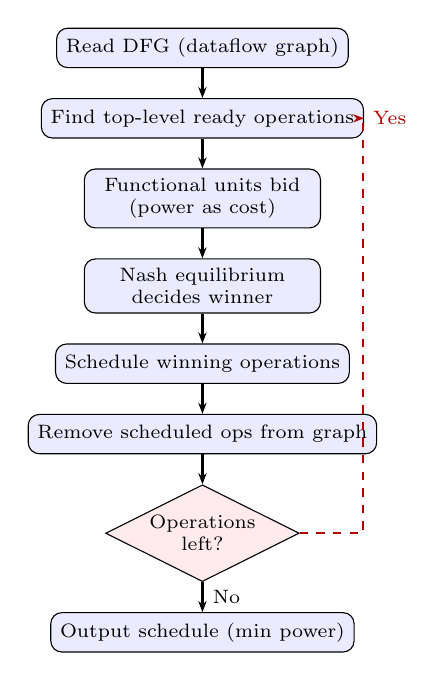
\begin{tikzpicture}[
  box/.style={rectangle,draw,rounded corners,fill=blue!8,minimum width=3.0cm,minimum height=0.5cm,font=\scriptsize,align=center},
  dec/.style={diamond,draw,fill=red!8,aspect=2,inner sep=1pt,font=\scriptsize,align=center},
  arr/.style={-{Stealth[length=4pt]},thick},
  fb/.style={-{Stealth[length=4pt]},thick,dashed,color=red!70!black},
  node distance=0.38cm]
  \node[box](read){Read DFG (dataflow graph)};
  \node[box,below=of read](top){Find top-level ready operations};
  \node[box,below=of top](bid){Functional units bid\\(power as cost)};
  \node[box,below=of bid](nash){Nash equilibrium\\decides winner};
  \node[box,below=of nash](sched){Schedule winning operations};
  \node[box,below=of sched](rem){Remove scheduled ops from graph};
  \node[dec,below=of rem](dec){Operations\\left?};
  \node[box,below=of dec](out){Output schedule (min power)};
  \draw[arr](read)--(top);\draw[arr](top)--(bid);\draw[arr](bid)--(nash);
  \draw[arr](nash)--(sched);\draw[arr](sched)--(rem);\draw[arr](rem)--(dec);
  \draw[arr](dec)--node[right,font=\scriptsize]{No}(out);
  \draw[fb](dec.east)--++(0.8,0)|-(top.east)node[midway,right,font=\scriptsize,color=red!70!black]{Yes};
\end{tikzpicture}
\caption{Flow of the game theoretic scheduling process. Bidding and the
Nash equilibrium are applied level by level until all operations are
scheduled.}
\label{fig:flow}
\end{figure}

For binding, the same idea is applied at each control step: the
compatible modules for a step are identified, a payoff matrix is built
from their power costs, and the Nash equilibrium selects the binding
that minimizes total power. The combined scheduling and binding
formulation applies the Nash equilibrium only once, using a single
unified payoff matrix, and achieves better power reduction than
applying scheduling and binding separately in
sequence~\cite{murugavel2003}.

% ============================================================
\section{Experimental Results}

The benchmark circuits used for evaluation are the differential
equation (Diff.\ eqn), finite impulse response filter (FIR), infinite
impulse response filter (IIR), and the larger lattice, elliptic wave
filter (EWF), WAVE, and noise-cancel filter (NC filter). Power values
were obtained by simulation with 100\,000 random 16-bit two's
complement input vectors using TSMC $0.25\,\mu\mathrm{m}$ cells, and
interconnect lengths were estimated using Rent's
rule~\cite{murugavel2003}. The results below are drawn from the
benchmark tables of Murugavel and Ranganathan and are used here to
support the approach.

\begin{table}[t]
\caption{Scheduling: Power (mW) and \% Improvement over ILP~\cite{murugavel2003}}
\label{tab:sched}
\centering
\footnotesize
\begin{tabular}{lccc}
\toprule
Circuit & ILP $P_{\mathrm{ILP}}$ & GT $P_{\mathrm{GT}}$ & Impr. \\
\midrule
Diff.\ eqn & 24.8 & 23.9 & 3.6\% \\
FIR & 82.8 & 78.7 & 4.9\% \\
IIR & 15.6 & 14.8 & 5.1\% \\
Lattice & 91.3 & 82.9 & 9.2\% \\
EWF & 262.8 & 251.0 & 4.5\% \\
WAVE & 258.2 & 232.8 & 9.8\% \\
NC filter & 389.7 & 363.4 & 6.7\% \\
\midrule
\textbf{Average} & & & \textbf{6.3\%} \\
\bottomrule
\end{tabular}
\end{table}

\begin{table}[t]
\caption{Binding: Power (mW) and \% Improvement over LP~\cite{murugavel2003}}
\label{tab:bind}
\centering
\footnotesize
\begin{tabular}{lccc}
\toprule
Circuit & LP $P_{\mathrm{LP}}$ & GT $P_{\mathrm{GT}}$ & Impr. \\
\midrule
Diff.\ eqn & 22.9 & 20.1 & 12.2\% \\
FIR & 72.0 & 57.7 & 19.8\% \\
IIR & 15.5 & 12.3 & 20.6\% \\
Lattice & 71.9 & 64.1 & 10.8\% \\
EWF & 234.3 & 210.0 & 10.4\% \\
WAVE & 215.1 & 196.3 & 8.7\% \\
NC filter & 368.5 & 312.8 & 15.1\% \\
\midrule
\textbf{Average} & & & \textbf{13.9\%} \\
\bottomrule
\end{tabular}
\end{table}

\begin{table}[t]
\caption{Combined Scheduling and Binding: Power (mW) and \% Improvement over ILP~\cite{murugavel2003}}
\label{tab:comb}
\centering
\footnotesize
\begin{tabular}{lccc}
\toprule
Circuit & ILP $P_{\mathrm{ILP}}$ & GT $P_{\mathrm{GT}}$ & Impr. \\
\midrule
Diff.\ eqn & 22.9 & 16.0 & 8.0\% \\
FIR & 61.7 & 50.4 & 18.3\% \\
IIR & 12.8 & 11.2 & 12.5\% \\
Lattice & 66.3 & 55.9 & 15.7\% \\
EWF & 204.0 & 191.3 & 6.2\% \\
WAVE & 201.2 & 179.2 & 10.9\% \\
NC filter & 324.3 & 286.7 & 11.5\% \\
\midrule
\textbf{Average} & & & \textbf{11.8\%} \\
\bottomrule
\end{tabular}
\end{table}

As shown in Table~\ref{tab:sched}, the game theoretic scheduling
algorithm yields an average improvement of about 6.3\% over the ILP
method, with run times comparable to ILP. The binding results in
Table~\ref{tab:bind} show an average improvement of about 13.9\% over
the LP-based technique, with the largest single-circuit gain on the IIR
filter at 20.6\%; this gain is achieved even without interconnect power
optimization, because the Nash equilibrium optimizes for all players
and because both functional unit and register binding are considered.
The combined scheduling and binding results in Table~\ref{tab:comb}
show an average improvement of about 11.8\% over the sequential
ILP-plus-LP baseline, with a worst-case latency increase of no more
than two cycles. Across all benchmarks there is no increase in area,
and run times remain comparable to the baselines.

% ============================================================
\section{Tradeoff Analysis}

The approach involves several tradeoffs. In the \emph{power versus
latency} tradeoff, power is the primary objective and latency is not
co-optimized, so the cost is a small latency increase of at most about
two cycles, which is acceptable for power-critical, throughput-tolerant
designs. In the \emph{power versus area} tradeoff, no additional
modules or multiplexers are introduced, so there is no area overhead,
and multiplexer power varies only minimally with the binding solution.
In the \emph{quality versus runtime} tradeoff, the Nash equilibrium is
NP-complete in general, but restricting the number of players to a few
units per type (typically two or three) per game keeps run times
comparable to ILP and LP. Finally, in the \emph{scheduling-only versus
combined} tradeoff, the combined formulation applies the Nash
equilibrium once and gives better power reduction than the separate
formulation, at the cost of a more intricate unified payoff matrix.

% ============================================================
\section{Advantages and Limitations}

The proposed game theoretic technique has several key advantages for
power optimization in HLS. Operations are extracted from the DFG and
each functional unit is treated as a player. Each participant
determines the operation it can perform with the least power
expenditure, and the Nash equilibrium then yields the assignment that
minimizes the power consumption at the functional unit for each
operation. This decreases the switching activity at the functional
units and thus minimizes overall power consumption. A further advantage
is that this strategy does not increase the hardware area; no new
adders, multipliers, or other functional units are added to the design.
Instead, the existing hardware components are used more efficiently
through better scheduling and binding, so the hardware area is
essentially unchanged and only the assignment of operations to units is
optimized.

The approach also has certain limitations. Because it prioritizes
minimizing power consumption rather than optimizing latency, additional
control cycles may sometimes be required, which can cause a slight
increase in delay. In addition, when the number of operations and
functional units becomes large, computing the Nash equilibrium becomes
more difficult, since a greater number of combinations must be checked,
which can make the technique slow~\cite{murugavel2003}.

% ============================================================
\section{Applications and Relevance}

This strategy is very beneficial for IoT devices, wearables, and mobile
devices, because the batteries in these devices are small and the power
constraints are highly strict. Lower power means longer battery life,
less heat, and better device efficiency. HLS makes hardware design
easier, and game theory together with the Nash equilibrium can be used
to allocate operations to functional units with lower power
consumption, which makes scheduling and binding decisions more
systematic. Looking ahead, if artificial intelligence or machine
learning is applied, the system can learn from prior design experience.
This would allow more intelligent judgments about which hardware unit
consumes less power, where latency can be reduced, and how computation
time can be minimized for larger circuits.

% ============================================================
\section{Future Work}

In this work, the main focus is on reducing power consumption. In
practical hardware design, however, low power and good speed are
equally vital; if only power is reduced, the circuit may become slow.
Extending this approach to jointly optimize power and latency is
therefore an interesting topic for future exploration. In addition,
interconnect binding should be taken into account, because in current
chips the power consumption and delay arise not only from functional
units but also from wires and interconnects, and the optimization is
not complete without considering them. Finally, computing the Nash
equilibrium requires much more time for large circuits with many
operations and hardware components; to address this, further study can
examine faster algorithms, heuristic approaches, search-space reduction
methods, or AI and machine learning based approaches that reduce the
computation time.

% ============================================================
\section{Conclusion}

This paper has presented a game theoretic approach to the scheduling
and binding problem in High-Level Synthesis. By modeling functional
units as players in a first-price sealed-bid auction and applying the
Nash equilibrium, operations are assigned to suitable functional units
in a way that minimizes power consumption without increasing the
hardware area. Benchmark data indicate average power improvements of
about 6.3\% for scheduling, 13.9\% for binding, and 11.8\% for combined
scheduling and binding over conventional baselines, at the cost of only
a slight latency increase. The main remaining challenges are the
scalability of the Nash equilibrium for large circuits and the absence
of an interconnect model. Future work should therefore focus on
reducing latency alongside power, incorporating interconnect binding,
and making the equilibrium computation faster, so that the approach can
be applied effectively to larger and more modern designs.

% ============================================================
\begin{thebibliography}{00}
\bibitem{murugavel2003}
A.~K.~Murugavel and N.~Ranganathan, ``A game theoretic approach for power optimization during behavioral synthesis,'' \textit{IEEE Trans.\ Very Large Scale Integr.\ (VLSI) Syst.}, vol.~11, no.~6, pp.~1031--1043, Dec.\ 2003.
\bibitem{shiue2000}
W.~T.~Shiue and C.~Chakrabarti, ``ILP-based scheme for low-power scheduling and resource binding,'' in \textit{Proc.\ Int.\ Symp.\ Circuits and Systems}, vol.~3, 2000, pp.~279--282.
\bibitem{small1994}
C.~Small, ``Shrinking devices put the squeeze on system packaging,'' \textit{Electron.\ Design News}, vol.~39, pp.~41--46, Feb.\ 1994.
\bibitem{benini2000}
L.~Benini and G.~De~Micheli, ``System-level power optimization: Techniques and tools,'' \textit{ACM Trans.\ Design Automation of Electron.\ Syst.}, vol.~5, no.~2, pp.~115--192, Apr.\ 2000.
\bibitem{gajski1992}
D.~Gajski, N.~Dutt, A.~Wu, and Y.-L.~Lin, \textit{High-Level Synthesis: Introduction to Chip and System Design}. Norwell, MA: Kluwer, 1992.
\bibitem{paulin1989}
P.~G.~Paulin and J.~P.~Knight, ``Scheduling and binding algorithms for high-level synthesis,'' in \textit{Proc.\ Design Automation Conf.}, 1989, pp.~1--6.
\bibitem{mohanty2003}
S.~P.~Mohanty, N.~Ranganathan, and S.~K.~Chappidi, ``Simultaneous peak and average power minimization during datapath scheduling for DSP processors,'' in \textit{Proc.\ Great Lakes Symp.\ VLSI}, 2003, pp.~215--220.
\bibitem{dasgupta1995}
A.~Dasgupta and R.~Karri, ``Simultaneous scheduling and binding for power minimization during micro-architecture synthesis,'' in \textit{Proc.\ Int.\ Symp.\ Low-Power Electronics Design}, 1995, pp.~69--74.
\bibitem{nash1951}
J.~F.~Nash, ``Non-cooperative games,'' \textit{Ann.\ Math.}, vol.~54, no.~2, pp.~286--295, 1951.
\bibitem{owen1995}
G.~Owen, \textit{Game Theory}, 3rd ed. New York: Academic, 1995.
\bibitem{friedman1990}
J.~W.~Friedman, \textit{Game Theory with Applications to Economics}. London, U.K.: Oxford Univ.\ Press, 1990.
\bibitem{park1988}
N.~Park and A.~C.~Parker, ``Sehwa: A software package for synthesis of pipelines from behavioral specifications,'' \textit{IEEE Trans.\ Computer-Aided Design}, vol.~7, pp.~356--370, Mar.\ 1988.
\bibitem{gambit2002}
R.~D.~McKelvey, A.~McLennan, and T.~Turocy, \textit{Gambit: Software Tools for Game Theory}, ver.\ 0.97, 2002.
\end{thebibliography}

\end{document}
